% Defining the document class and necessary packages
\documentclass{article}
\usepackage{tikz}
\usetikzlibrary{patterns}
\usepackage{pgfplots}
\pgfplotsset{compat=1.18}
\usepackage{noto}
\usepackage{geometry}
\geometry{letterpaper, margin=1.25cm}

\usepackage{graphicx} % For including figures
\usepackage{xcolor} % For color support
\usepackage{caption} % For customizing captions
\usepackage{hyperref} % For hyperlinks


% Configuring hyperref for link styling
\hypersetup{
    colorlinks=true, % Use colored links instead of boxes
    linkcolor=blue, % Color for internal links (e.g., figure references)
    citecolor=blue, % Color for citations
    urlcolor=blue % Color for URLs
}

% Customizing figure caption style
\captionsetup[figure]{
    labelfont={bf, color=blue}, % Bold and blue figure labels
    textfont={color=black}, % Caption text remains black
    %labelsep=period % Period after "Figure X"
}

\captionsetup[table]{
    labelfont={bf, color=blue}, % Bold and blue figure labels
    textfont={color=black}, % Caption text remains black
    %labelsep=period % Period after "Figure X"
}


% Starting the document
\begin{document}

% Creating a 2x2 grid of charts using minipage
\begin{figure}[ht]
\centering

% Top row, first chart (Case 1)
\begin{minipage}{0.48\textwidth}
\centering
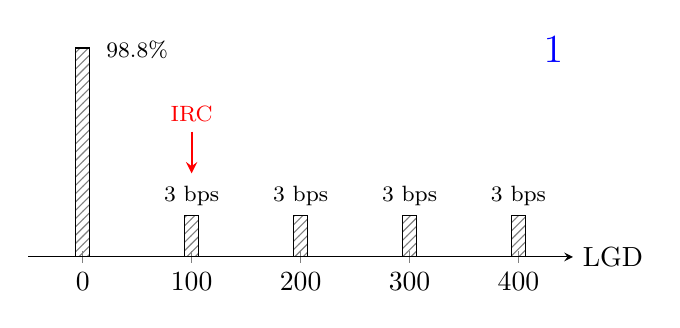
\begin{tikzpicture}
\begin{axis}[
    width=8.5cm,
    height=4.5cm,
    axis x line=middle,
    axis y line=none,
    xlabel={LGD},
    xlabel style={at={(axis cs:4.5,0)}, anchor=west},
    ylabel={},
    xtick={0,1,2,3,4},
    xticklabels={0,100,200,300,400},
    ytick=\empty,
    yticklabels=\empty,
    ymin=0, ymax=11,
    xmin=-0.5, xmax=4.5,
    bar width=0.18cm,
]
\addplot[
    ybar,
    fill=gray,
    fill opacity=0.5,
    draw=black,
    pattern=north east lines,
    pattern color=gray
] coordinates {
    (0,10) (1,2) (2,2) (3,2) (4,2)
};
\node[above, font=\footnotesize] at (axis cs:0.5,9) {98.8\%};
\node[above, font=\footnotesize] at (axis cs:1,2) {3 bps};
\node[above, font=\footnotesize] at (axis cs:2,2) {3 bps};
\node[above, font=\footnotesize] at (axis cs:3,2) {3 bps};
\node[above, font=\footnotesize] at (axis cs:4,2) {3 bps};
\draw[red, -stealth, thick] (axis cs:1,6) -- (axis cs:1,4);
\node[above, font=\footnotesize, red] at (axis cs:1,6) {IRC};
\node[font=\normalsize, anchor=north east] at (axis cs:4.5,11) {\textcolor{blue}{\Large 1}};
\end{axis}
\end{tikzpicture}
\end{minipage}
\hfill
% Top row, second chart (Case 2)
\begin{minipage}{0.48\textwidth}
\centering
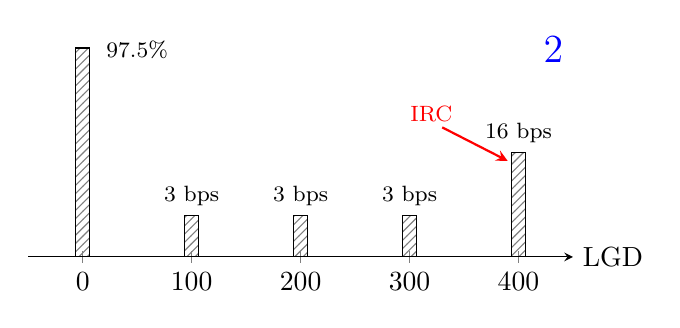
\begin{tikzpicture}
\begin{axis}[
    width=8.5cm,
    height=4.5cm,
    axis x line=middle,
    axis y line=none,
    xlabel={LGD},
    xlabel style={at={(axis cs:4.5,0)}, anchor=west},
    ylabel={},
    xtick={0,1,2,3,4},
    xticklabels={0,100,200,300,400},
    ytick=\empty,
    yticklabels=\empty,
    ymin=0, ymax=11,
    xmin=-0.5, xmax=4.5,
    bar width=0.18cm,
]
\addplot[
    ybar,
    fill=gray,
    fill opacity=0.5,
    draw=black,
    pattern=north east lines,
    pattern color=gray
] coordinates {
    (0,10) (1,2) (2,2) (3,2) (4,5)
};
\node[above, font=\footnotesize] at (axis cs:0.5,9) {97.5\%};
\node[above, font=\footnotesize] at (axis cs:1,2) {3 bps};
\node[above, font=\footnotesize] at (axis cs:2,2) {3 bps};
\node[above, font=\footnotesize] at (axis cs:3,2) {3 bps};
\node[above, font=\footnotesize] at (axis cs:4,5) {16 bps};
\draw[red, -stealth, thick] (axis cs:3.3,6.2) -- (axis cs:3.9,4.6);
\node[above, font=\footnotesize, red] at (axis cs:3.2,6) {IRC};
\node[font=\normalsize, anchor=north east] at (axis cs:4.5,11) {\textcolor{blue}{\Large 2}};
\end{axis}
\end{tikzpicture}
\end{minipage}

\vspace{1cm}

% Bottom row, first chart (Case 3)
\begin{minipage}{0.48\textwidth}
\centering
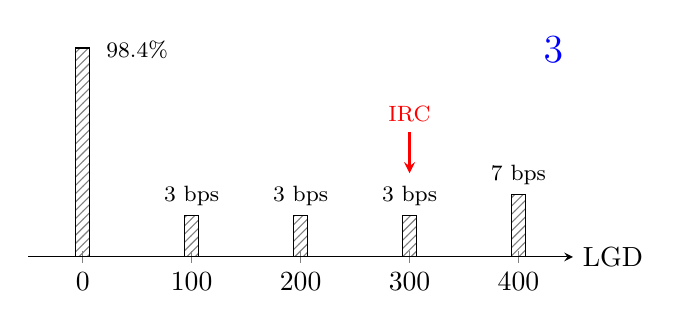
\begin{tikzpicture}
\begin{axis}[
    width=8.5cm,
    height=4.5cm,
    axis x line=middle,
    axis y line=none,
    xlabel={LGD},
    xlabel style={at={(axis cs:4.5,0)}, anchor=west},
    ylabel={},
    xtick={0,1,2,3,4},
    xticklabels={0,100,200,300,400},
    ytick=\empty,
    yticklabels=\empty,
    ymin=0, ymax=11,
    xmin=-0.5, xmax=4.5,
    bar width=0.18cm,
]
\addplot[
    ybar,
    fill=gray,
    fill opacity=0.5,
    draw=black,
    pattern=north east lines,
    pattern color=gray
] coordinates {
    (0,10) (1,2) (2,2) (3,2) (4,3)
};
\node[above, font=\footnotesize] at (axis cs:0.5,9) {98.4\%};
\node[above, font=\footnotesize] at (axis cs:1,2) {3 bps};
\node[above, font=\footnotesize] at (axis cs:2,2) {3 bps};
\node[above, font=\footnotesize] at (axis cs:3,2) {3 bps};
\node[above, font=\footnotesize] at (axis cs:4,3) {7 bps};
\draw[red, -stealth, thick] (axis cs:3,6) -- (axis cs:3,4);
\node[above, font=\footnotesize, red] at (axis cs:3,6) {IRC};
\node[font=\normalsize, anchor=north east] at (axis cs:4.5,11) {\textcolor{blue}{\Large 3}};
\end{axis}
\end{tikzpicture}
\end{minipage}
\hfill
% Bottom row, second chart (Case 4)
\begin{minipage}{0.48\textwidth}
\centering
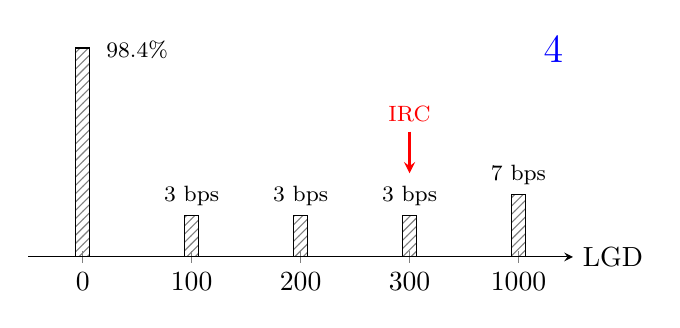
\begin{tikzpicture}
\begin{axis}[
    width=8.5cm,
    height=4.5cm,
    axis x line=middle,
    axis y line=none,
    xlabel={LGD},
    xlabel style={at={(axis cs:4.5,0)}, anchor=west},
    ylabel={},
    xtick={0,1,2,3,4},
    xticklabels={0,100,200,300,1000},
    ytick=\empty,
    yticklabels=\empty,
    ymin=0, ymax=11,
    xmin=-0.5, xmax=4.5,
    bar width=0.18cm,
]
\addplot[
    ybar,
    fill=gray,
    fill opacity=0.5,
    draw=black,
    pattern=north east lines,
    pattern color=gray
] coordinates {
    (0,10) (1,2) (2,2) (3,2) (4,3)
};
\node[above, font=\footnotesize] at (axis cs:0.5,9) {98.4\%};
\node[above, font=\footnotesize] at (axis cs:1,2) {3 bps};
\node[above, font=\footnotesize] at (axis cs:2,2) {3 bps};
\node[above, font=\footnotesize] at (axis cs:3,2) {3 bps};
\node[above, font=\footnotesize] at (axis cs:4,3) {7 bps};
\draw[red, -stealth, thick] (axis cs:3,6) -- (axis cs:3,4);
\node[above, font=\footnotesize, red] at (axis cs:3,6) {IRC};
\node[font=\normalsize, anchor=north east] at (axis cs:4.5,11) {\textcolor{blue}{\Large 4}};
\end{axis}
\end{tikzpicture}
\end{minipage}
\caption{Distribution of Loss Given Default (LGD) across various scenarios, with probabilities displayed above each bar. The Incremental Risk Charge (IRC), representing the loss at the 99.9th percentile, is indicated by a red arrow. Figure not drawn to scale.}
\label{fig:IRC_cases}
\end{figure}
The Incremental Risk Charge (IRC) is defined as the 99.9th percentile of the loss distribution, meaning it captures losses up to this threshold but excludes those in the extreme tail beyond it. Due to the discrete nature of losses from default or rating migration events for individual entities, IRC can be significantly impacted by high concentrations in a few entities, even if those entities are high quality with a low probability of default.

\section*{IRC Oddities}
To illustrate these characteristics of IRC, consider the four examples shown in
\autoref{fig:IRC_cases}:

\begin{enumerate}
\item The portfolio includes four entities, each with a 3 bps PD and loss given default (LGD) of 100, 200, 300, or 400. Ignoring rating migration and simultaneous defaults, the loss distribution is: 3 bps probability at each LGD, and 98.8\% (1 - 4$\times$ 3 bps) probability of no loss. The Incremental Risk Charge (IRC), which corresponds to the loss at the 99.9th percentile, is 100. Only the entity with LGD 100 contributes 100 to the IRC; others contribute zero;
\item If the entity with an LGD of 400 has a 16 bps probability of default instead, the IRC becomes 400, as the 99.9th percentile now falls within the loss of 400, which has a probability of 16 bps. The entire IRC is attributed to the entity with the LGD of 400;
\item If the entity with the LGD of 400 has a 7 bps PD, then the IRC will be 300, determined completely by the loss due to the default of the entity with LGD 300;
\item Increasing the LGD of the entity with a 7 bps PD to 1000 does not affect the IRC, although the risk profile of the portfolio has obviously changed.
\end{enumerate}

\begin{table}
\begin{center}

\begin{tabular}{rrrrrrrr} \hline \hline
%\toprule
$\rho$ & Aa & A & Baa & Ba & B & Caa & Ca\_C \\ \hline
%\midrule
5\% & 0.99963 & 0.99714 & 0.99717 & 0.99723 & 0.99728 & 0.99731 & 0.99740 \\
10\% & 0.99700 & 0.99705 & 0.99711 & 0.99720 & 0.99726 & 0.99732 & 0.99743 \\
15\% & 0.99691 & 0.99699 & 0.99706 & 0.99718 & 0.99728 & 0.99734 & 0.99747 \\
20\% & 0.99683 & 0.99693 & 0.99703 & 0.99718 & 0.99729 & 0.99737 & 0.99754 \\
25\% & 0.99677 & 0.99688 & 0.99700 & 0.99718 & 0.99732 & 0.99740 & 0.99758 \\
30\% & 0.99670 & 0.99683 & 0.99699 & 0.99720 & 0.99735 & 0.99744 & 0.99764 \\
35\% & 0.99664 & 0.99680 & 0.99699 & 0.99722 & 0.99738 & 0.99749 & 0.99770 \\
40\% & 0.99656 & 0.99676 & 0.99699 & 0.99725 & 0.99743 & 0.99755 & 0.99776 \\
%\bottomrule
\hline
\end{tabular}
\end{center}
\label{tab:ES_CI}
\caption{Confidence level for expected shortfall equivalent to VaR at 99.9\%.}
\end{table}


% Ending the document
\end{document}